\section{XACML Policy Refactoring Process} \label{sec:approach}
This section describes our approach of refactoring access control policies to improve performance by reducing the number of policy rules potentially applicable to the request.
For refactoring policies in a systematic way, we propose seven policy splitting criteria based on attribute set. 
Moreover, we explain how to select the splitting criterion, which preserves the synergy in the access control architecture.

\subsection{Definition of Policy based Splitting Criteria} \label{subsec:SplittingCriteria}
Given a request, a PDP uses brute force searching to retrieve the decision, by evaluating the request against all the policy rules. 
For request evaluation processing, not of all the rules are applicable to the request.
In other words, only part of the rules (i.e., relevant rules) are applicable to the request and contribute
to build the final authorization decision. We propose an approach to evaluate a request against only the relevant rules for a given request by refactoring
access control policies. Our approach aims at splitting a single global policy into multiple smaller policies based on attribute values combination. 
For a given policy-based system, we transform the policy \normalsize $P$ into 
policies \normalsize $P_{SC_{w}}$ containing less number of rules and conforming to a Splitting Criteria $SC_{w}$. 
An $SC_{w}$ defines the set of attributes that are considered 
to classify all the rules into subsets having similar one or more attribute values, $w$ denotes the number of attributes that have to be considered conjointly 
for aggregating rules based on specific attribute elements selection. Table \ref{table1} shows our proposed splitting criteria categories according to
 the attribute elements combination.

\begin{table}[h!]
\centering
\setlength{\extrarowheight}{6 pt}
\begin{tabular}{|>{\small}c|>{\small}c|}
\hline \rowcolor{black}
\bf
\textcolor{white}{Categories}& \bf \textcolor{white}{Splitting Criteria}\\ \hline
$SC_{1}$& {$\langle Subject \rangle, \langle Resource\rangle, \langle Action\rangle$}\\ \hline
$SC_{2}$& {$\langle Subject,Action \rangle, \langle Subject,Resource\rangle$}\\&{$\langle Resource,Action\rangle$}\\ \hline
$SC_{3}$& {$\langle Subject,Resource,Action\rangle$}\\ \hline
\end{tabular}
\caption{Splitting Criteria}
\label{table1}\end{table}



Figure \ref{splitting} presents a splitting process example in which an XACML policy $P$ is refcatored according to
 the splitting criterion $SC_{1}=\langle Subject\rangle$. The refactoring results in two sub-policies $Pa$ and $Pb$ where
each consists in rules having respectively the same subject (Alice or Bob in this case).

\begin{figure}[!h]
\begin{center}
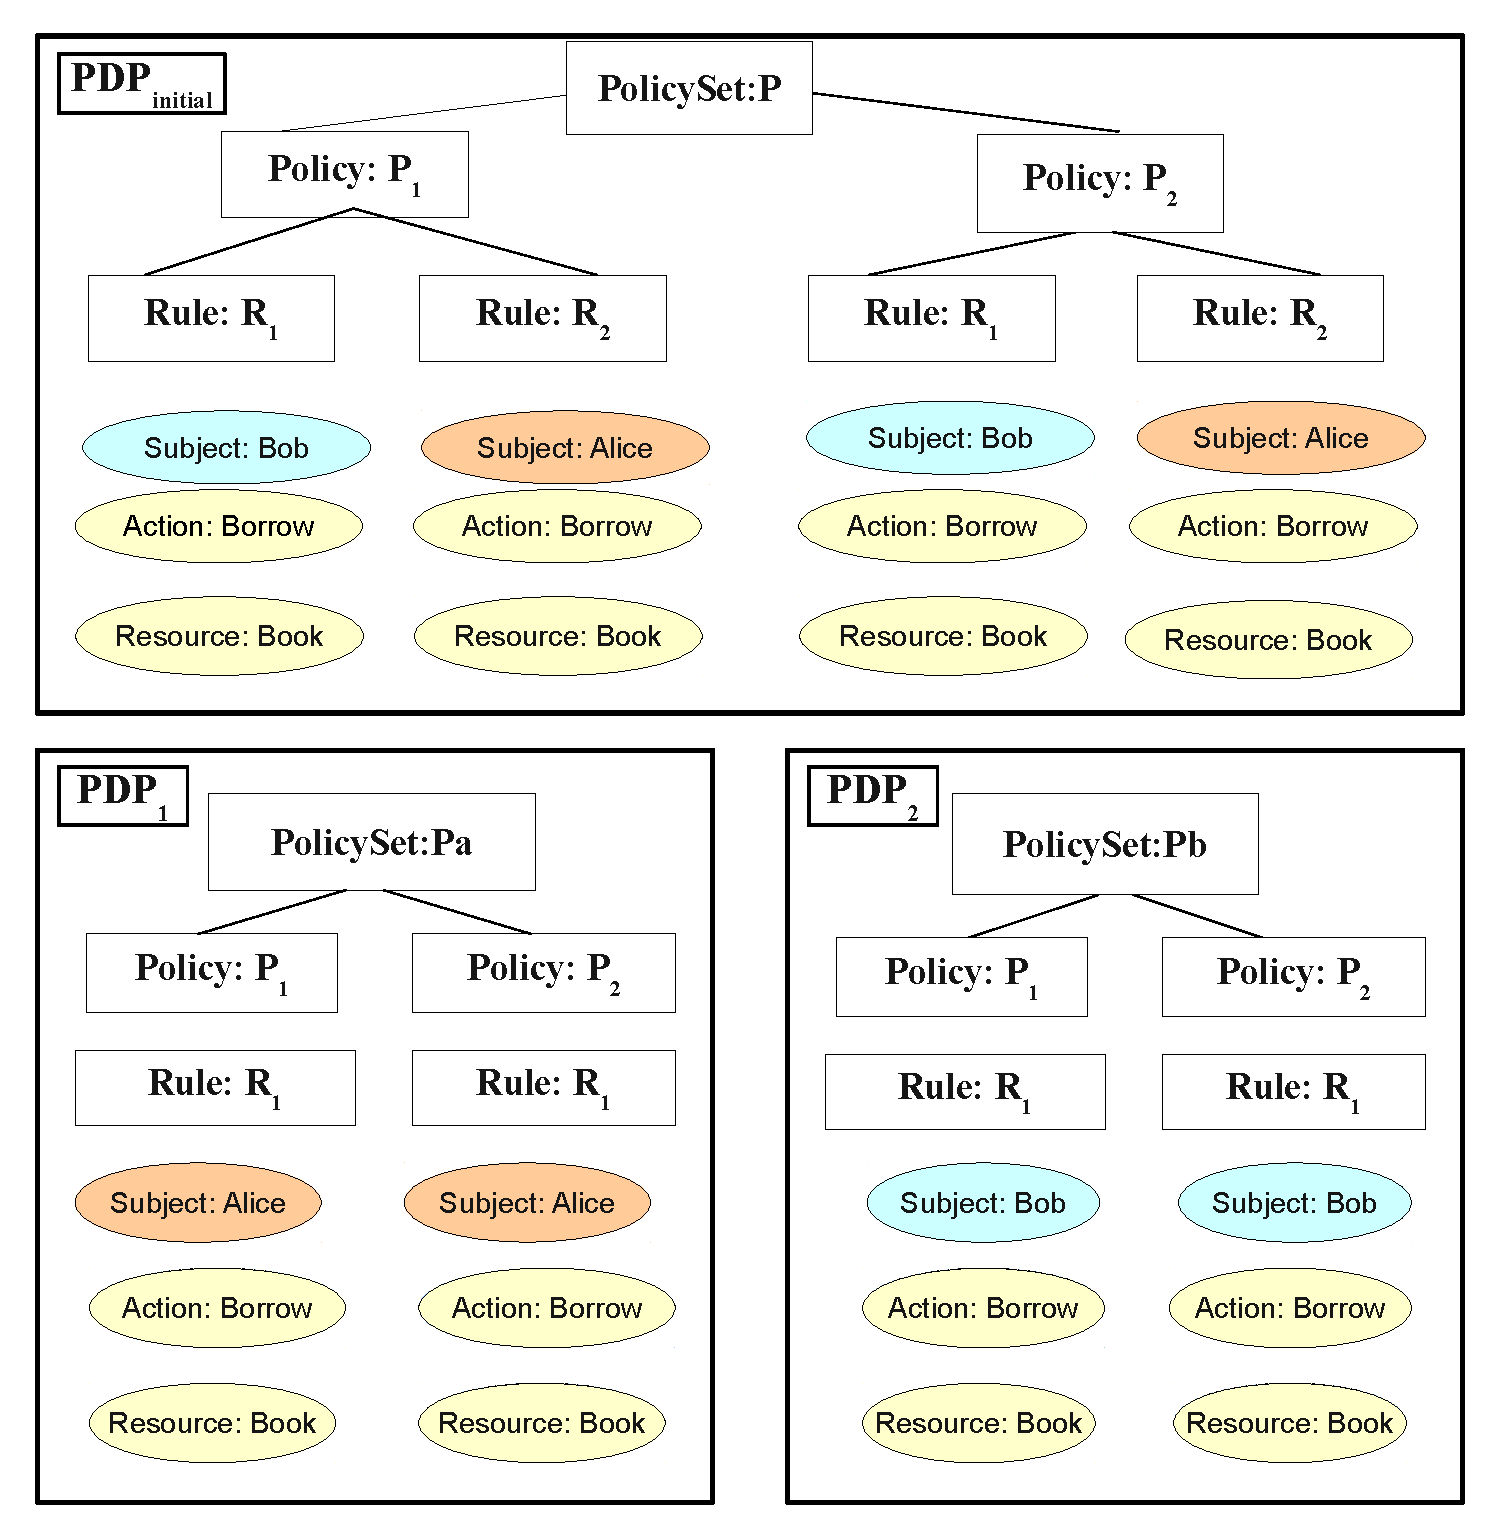
\includegraphics[width=8.5cm, height=9cm]{splitting}
\caption{XACML policy refactoring according to $SC_{1}=\langle Subject\rangle$}
\label{splitting}
\end{center}
\end{figure}

The Algorithm below illustrates the splitting process for $SC_{1}=\langle Subject\rangle$.
\begin{algorithmic}
\begin{algorithm}[!h]
\caption{Policy Splitting Algorithm}
\STATE \textbf{Input:} XACML Policy $P$, Splitting Criteria $SC_{1}$=$\langle Subject \rangle$
\STATE \textbf{Output:} Sub-policies Set: S
\STATE \textbf{SplitPolicy()}
\STATE /* Collect all subjects in all the rules /*
\FORALL{$R_{i}\in P$}
\STATE /* Fetch all the targets to extract attributes collections depending on SC */
\FORALL{Target t in $R_{i}$}
\IF {t.contains(SubjectElement)}
\STATE SubjectCollection.add(SubjectElement.attribute)
\ENDIF
\ENDFOR
\ENDFOR
\STATE /* Build sub-policies based on subjects collected in SubjectCollection */
\FOR{int i = 0; i < SubjectCollection.size(); ++i}
\STATE /* Remove all the rules that do not contain SubjectCollection.at(i) in their Targets*/
\FORALL{$R_{i}\in P$}
\STATE  \textbf{BOOL} remove=TRUE


\FORALL{Target t in $R_{i}$}
\IF {t.SubjectElement.attribute in $R_{i}$ \textbf{equals} SubjectCollection.at(i)}
\STATE remove=FALSE
\ENDIF
\ENDFOR
\IF{ remove.equals(True)} \STATE{Remove $R_{i}$}  \ENDIF
\ENDFOR
\STATE /* $P_{(SubjectCollection.at(i))}$ is a sub-policy having only rules where the subjectAttribute is equals to SubjectCollection.at(i) */
\STATE $S=S+P_{(SubjectCollection.at(i))}$
\ENDFOR
\end{algorithm}
\end{algorithmic}



It is worth mentioning the following issues related to the refactoring process:
\begin{itemize}
\item
XACML supports multi-valued attributes in policies and requests. In XACML, \CodeIn{Target} elements define a set of attribute values, which match with the context element in
an access control request. In Figure~\ref{xacml-match}, subject attribute includes two attributes (one is "role" and the other is "isEq-subjUserId-resUserId"). In order to 
match the subject with multi-valued attributes, a request should include at least \CodeIn{pc-member} and \CodeIn{ture} for "role" and "isEq-subjUserId-resUserId", respectively.
Our approach considers such a whole subject element as a single entity, which is not splitted the policy splitter component.
\item XACML supports multi-valued attributes in policies and requests. For example, a subject in a given request could be both a manager role and a employee role. 
We don't consider multi-valued attributes in this paper.
\end{itemize}

\begin{figure}[!h]
\begin{center}
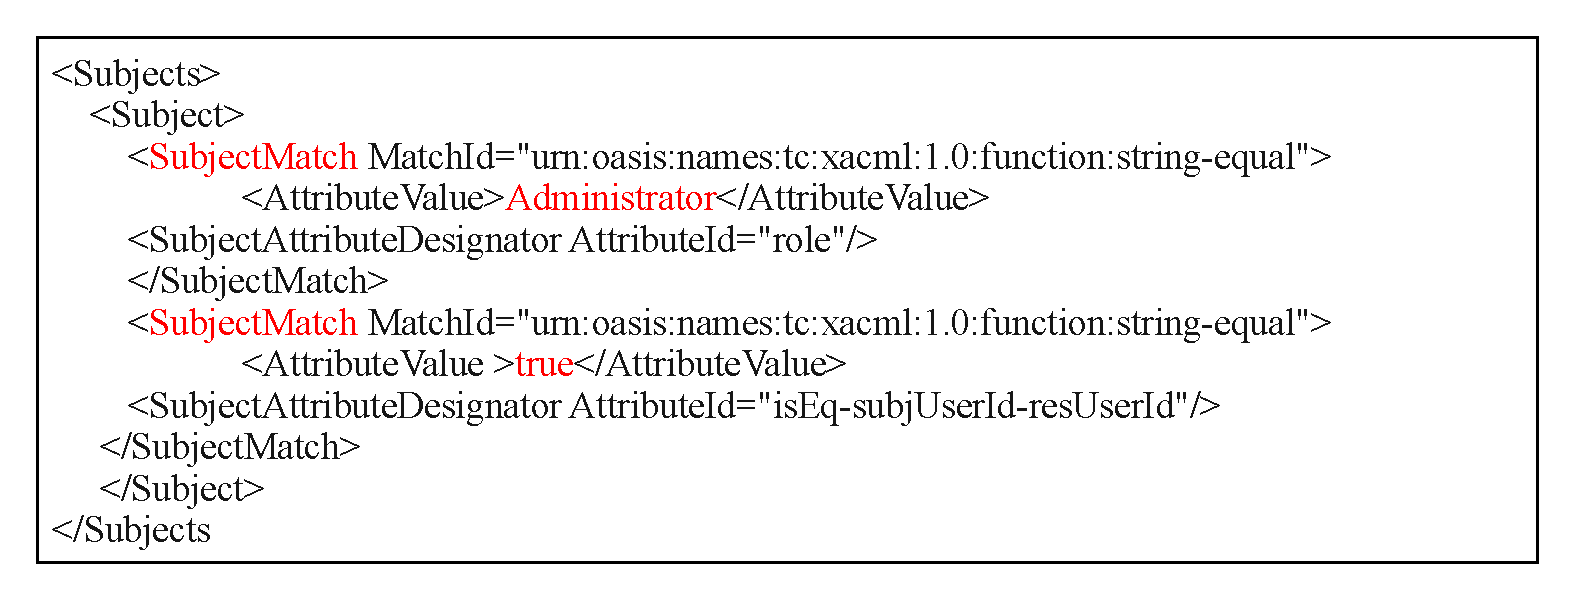
\includegraphics[width=9cm, height=3.5cm]{xacml-match}
\caption{Multi-attributes values in \CodeIn{target} element}
\label{xacml-match}
\end{center}
\end{figure}

After the splitting process is performed, our approach creates one or more (PDPs) that comply with a certain splitting criterion.
We use SUN PDP \cite{sunxacml} that evaluates requests against the policies specified in XACML.
During request evaluation, SUN PDP checks the request against the policy and determines whether its authorization
decision is permit or deny. Given a request, our approach fetches a SUN PDP loaded with the relevant policy, which is used during the decision making process. 
The PDP then retrieve the applicable rules that are applicable to the request.
Figure \ref{requestevaluation} presents our approach to handle request evaluation with multiple policies.
During the evaluation process, given a request, our approach verifies the matching between the request's attributes
and the policy set attributes. Our approach then selects only relevant policy among all of policies for a given request.
After the selection of the relevant policy, all of its relevant rules for the decision making are evaluated.


\begin{figure}[!h]
\begin{center}
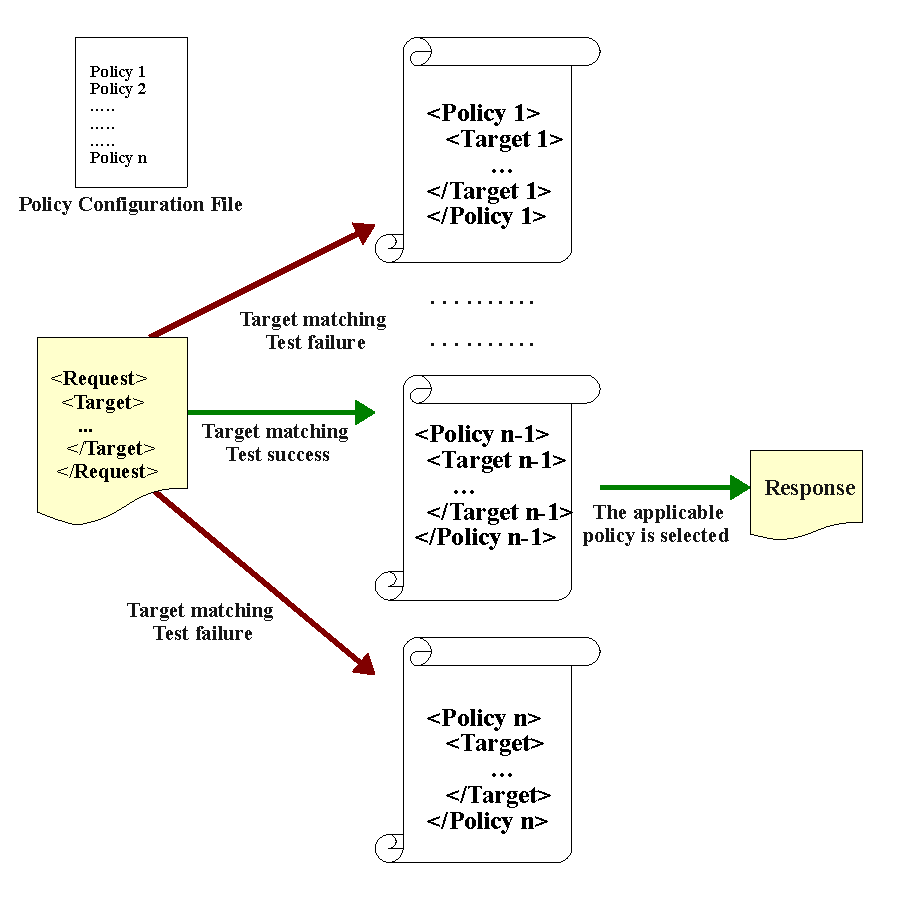
\includegraphics[width=3in, height=3in]{requestevaluation}
\caption{Applicable policy Selection}
\label{requestevaluation}
\end{center}
\end{figure}


Figure \ref{overallprocess} shows a general overview of the process. Given a single PDP loaded with initial global policy, the policy splitter 
tool conducts automated refactoring process by creating multiple PDPs loaded with XACML 
policies, which are split from the initial global policy based on user specified SC.
%Afterwards, the policies are included in the
%framework that supports our approach.
If the initial global policy is updated, the policy splitter is required to refactor the policy again to create PDPs with the most recent relevant 
policies. Our refactoring approach is safe in the sense that the approach does not impact existing functional aspects in a given
system.
\begin{figure}[!h]
\begin{center}
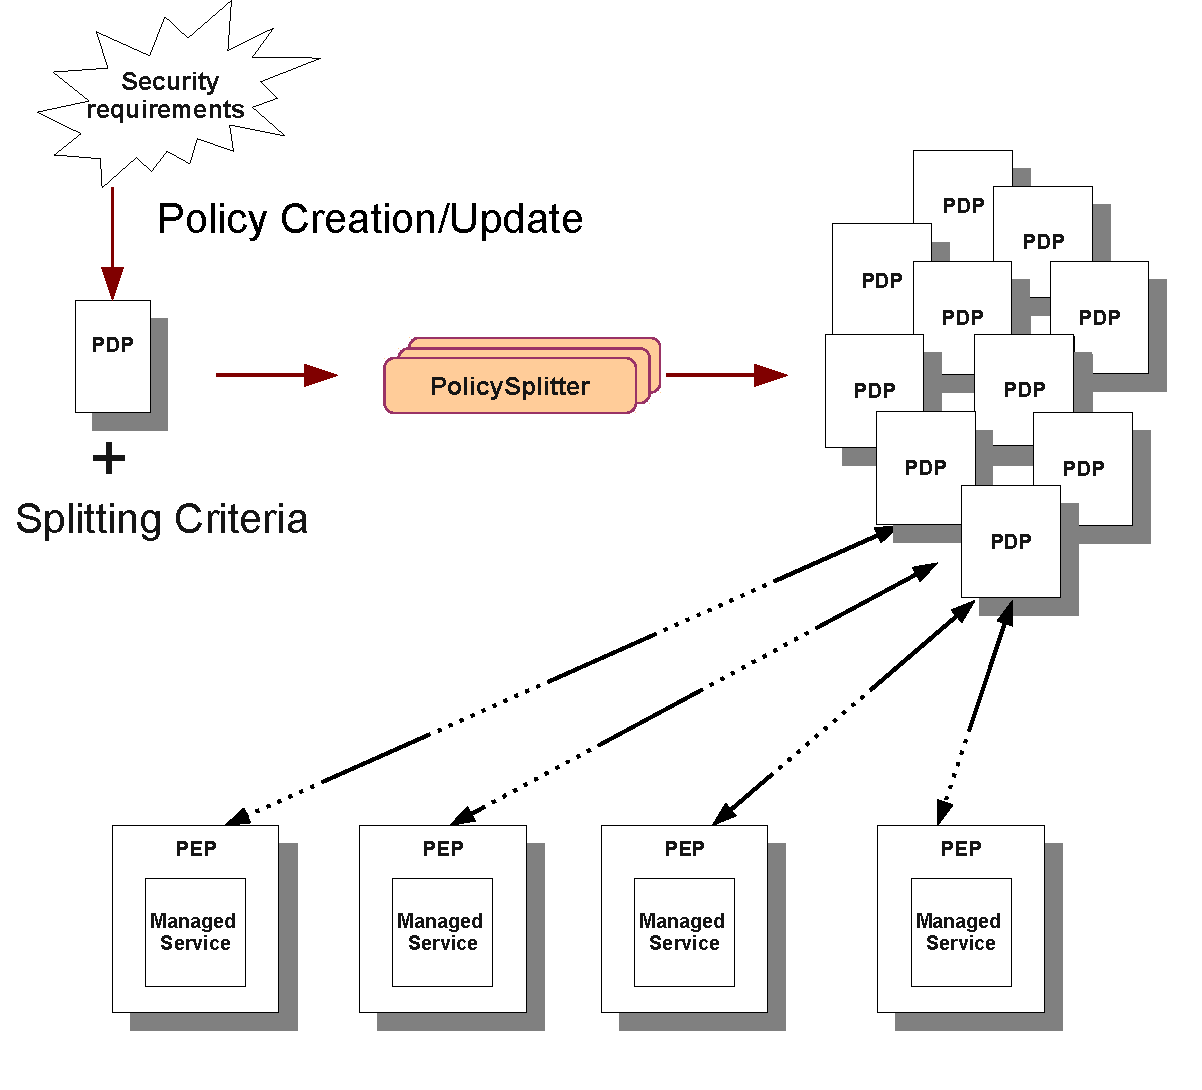
\includegraphics[width=8.5cm, height=8cm]{Overall-process}
\caption{Overview of the Refactoring Process}
\label{overallprocess}
\end{center}
\end{figure}



%Synergy Requirement for Access Control Architecture

\subsection{Architecture Model Preservation: PEP-PDP Synergy}
We consider the different splitting criteria that we have identified in the previous section and we propose to select the splitting criterion that 
enables to preserve the synergy in the access control architecture, this splitting criterion enables to have a valid refactoring and respects how PEPs are organized 
at the application level and how they are linked to their corresponding PDPs.
In the worst case, splitting the initial PDP into multi-PDPs may lead to a non-synergic system: a PEP may send its requests to several PDPs. 
The PDP, which receives a request is only known at runtime. Such a resulting architecture breaks the PEP-PDP synergy and the conceptual 
simplicity of the initial architecture model. In the best case, the refactoring preserves the simplicity of the initial architecture, by keeping a many-to-one association 
from PEPs to PDPs. A given request evaluation triggered by one PEP will always be handled by the same PDP. Operationally, the request evaluation process will involve 
one XACML policy file. In this case, the refactoring is valid, since its does not impact the conceptual architecture of the system.
Figure \ref{Synergic vs Non synergic System} presents a PDP encapsulating a global policy that has been refactored. The system that is presented in the left is a valid refactoring whereas 
the one in the right shows a non valid refactoring.
\begin{figure}[!h]
\begin{center}
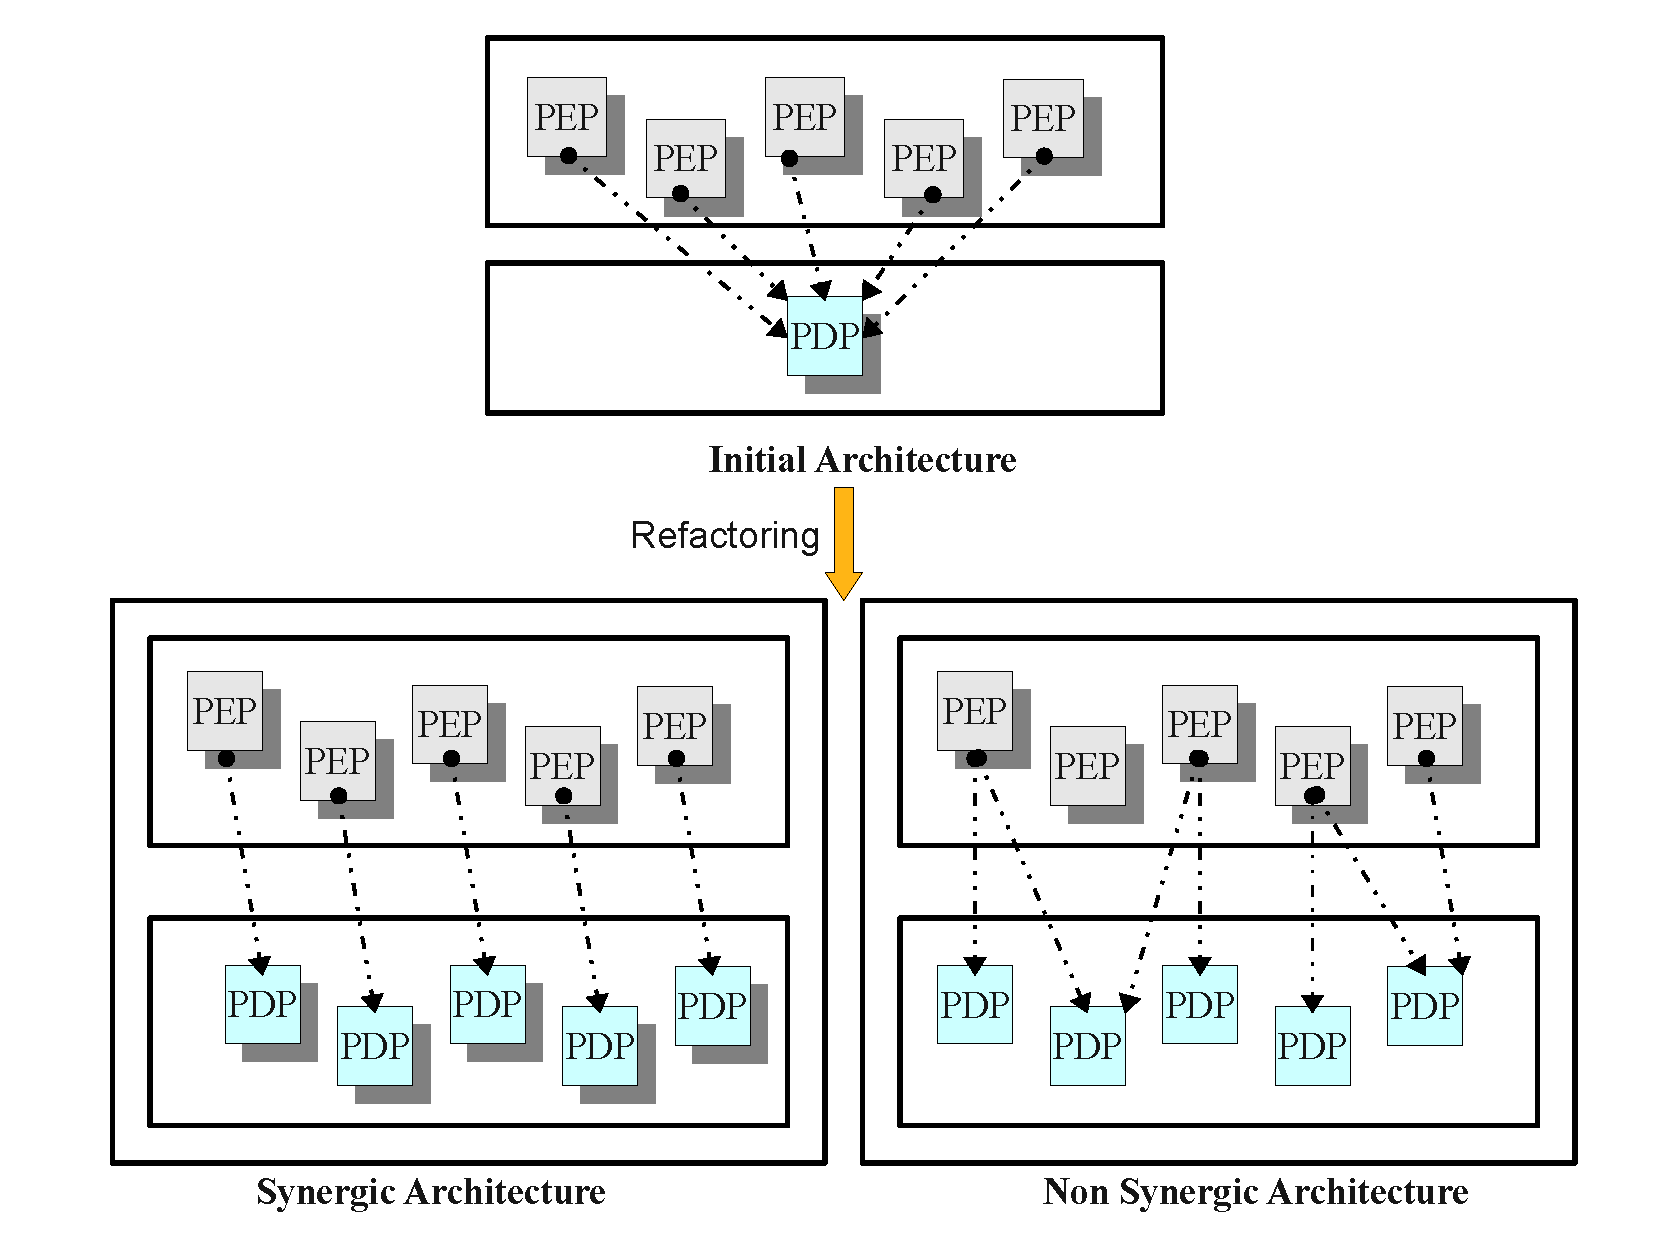
\includegraphics[width=8.5cm, height=6cm]{synergic-nonsynergic}
\caption{Synergic vs Non synergic System}
\label{Synergic vs Non synergic System}
\end{center}
\end{figure}
A deep analysis of the PEPs at the application enables to observe the mapping between the PEPs and the PDP. At the application level, the PEP
is represented by a method call that triggers a decision making process by activating some specific rules in the PDP.
The code in Figure \ref{PEP deployment Example} is taken from \cite{legacy}, this code excerpt shows an example of a PEP represented by the method checkSecurity which calls the class 
SecurityPolicyService that initiates the PDP component.

%An analysis of this code reflects that the PEP presented by the method ServiceUtils.checkSecurity will trigger exclusively all the rules 
%that have the subject user (provided as input parameter in the PEP) and fixed Action and Resource (LibrarySecurityModel.BORROWBOOK\_METHOD), ( LibrarySecurityModel.BOOK\_VIEW).


The PEP presented by the method \CodeIn{ServiceUtils.checkSecurity} may issue requests that have subject user role along fixed action and 
resource (``LibrarySecurityModel.BORROWBOOK\_METHOD''), (``LibrarySecurityModel.BOOK\_VIEW'').
Consider that we refactor a policy according to $SC_{2}=\langle Resource,Action\rangle$.
Give a request issued from the PEP, our approach fetches a PDP loaded with a policy containing rules having those action and resource attributes.
\begin{figure}[!h]
\begin{center}
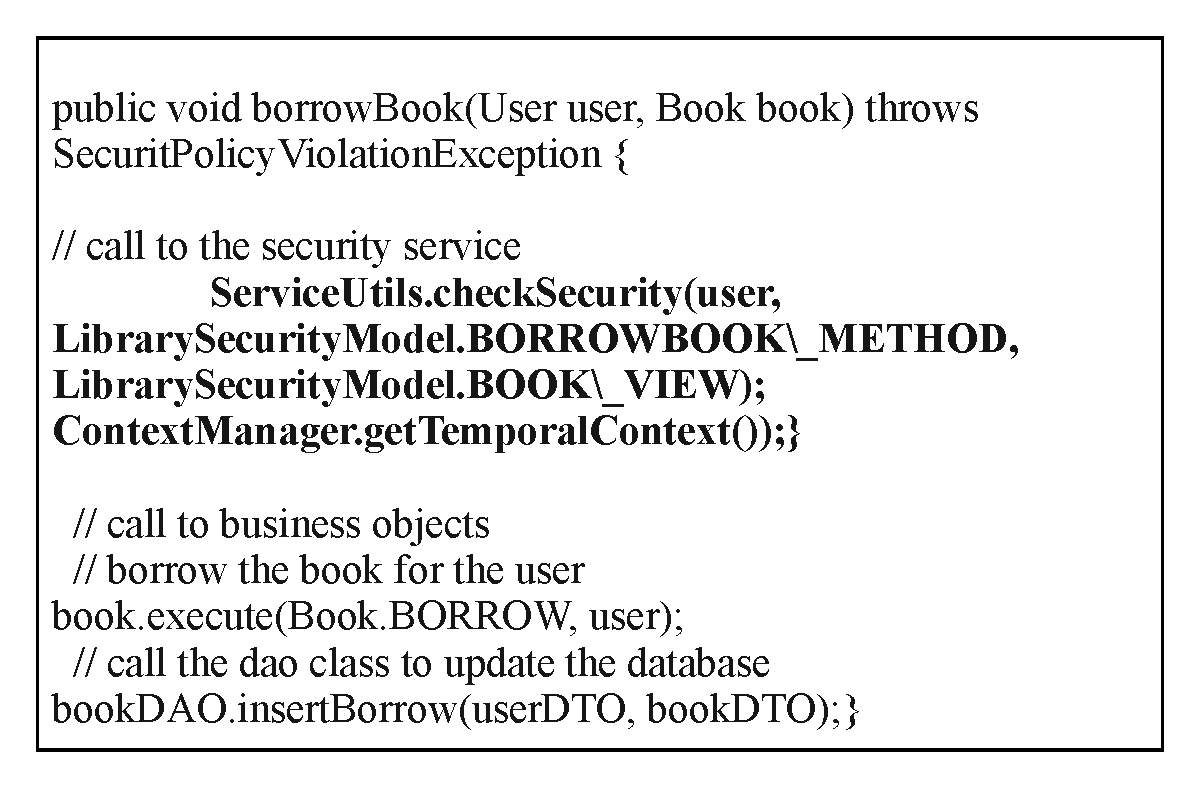
\includegraphics[width=7.5cm, height=4cm]{PEPExample}
\caption{PEP deployment Example}
\label{PEP deployment Example}
\end{center}
\end{figure}


Thus the splitting process that will preserve the mapping between the PEPs and the PDP is $SC_{2}=\langle Resource,Action\rangle$ since the rules in the policy are triggered 
by Action, Resource. Depending on the organization of the PEPs in a given application, connecting the rules with their PEPs at the application level may require to identify
 all the enforcements points in the application, and to track the different method calls triggered from these specific enforcement calls to map them to the relevant access
 control rules.

Our empirical results, presented in section~\ref{sec:experiment}, have shown that adopting a policy refactoring based on system functions, as a refactoring strategy, enables to 
have the best splitting criterion in term of performance. 
